%%%%%%%%%%%%%%%%%%%%%%%%%%%%%%%%%%%%%%%%%
% Beamer Presentation
% LaTeX Template
% Version 1.0 (10/11/12)
%
% This template has been downloaded from:
% http://www.LaTeXTemplates.com
%
% License:
% CC BY-NC-SA 3.0 (http://creativecommons.org/licenses/by-nc-sa/3.0/)
%
%%%%%%%%%%%%%%%%%%%%%%%%%%%%%%%%%%%%%%%%%

%----------------------------------------------------------------------------------------
%	PACKAGES AND THEMES
%----------------------------------------------------------------------------------------

\documentclass{beamer}

\mode<presentation> {

% The Beamer class comes with a number of default slide themes
% which change the colors and layouts of slides. Below this is a list
% of all the themes, uncomment each in turn to see what they look like.

%\usetheme{default}
%\usetheme{AnnArbor}
%\usetheme{Antibes}
%\usetheme{Bergen}
%\usetheme{Berkeley}
%\usetheme{Berlin}
%\usetheme{Boadilla}
%\usetheme{CambridgeUS}
%\usetheme{Copenhagen}
%\usetheme{Darmstadt}
%\usetheme{Dresden}
%\usetheme{Frankfurt}
%\usetheme{Goettingen}
%\usetheme{Hannover}
%\usetheme{Ilmenau}
%\usetheme{JuanLesPins}
%\usetheme{Luebeck}
%\usetheme{Madrid}
%\usetheme{Malmoe}
%\usetheme{Marburg}
%\usetheme{Montpellier}
%\usetheme{PaloAlto}
%\usetheme{Pittsburgh}
%\usetheme{Rochester}
%\usetheme{Singapore}
%\usetheme{Szeged}
%\usetheme{Warsaw}

% As well as themes, the Beamer class has a number of color themes
% for any slide theme. Uncomment each of these in turn to see how it
% changes the colors of your current slide theme.

%\usecolortheme{albatross}
%\usecolortheme{beaver}
%\usecolortheme{beetle}
%\usecolortheme{crane}
\usecolortheme{dolphin}
%\usecolortheme{dove}
%\usecolortheme{fly}
%\usecolortheme{lily}
%\usecolortheme{orchid}
%\usecolortheme{rose}
%\usecolortheme{seagull}
%\usecolortheme{seahorse}
%\usecolortheme{whale}
%\usecolortheme{wolverine}

%\setbeamertemplate{footline} % To remove the footer line in all slides uncomment this line
%\setbeamertemplate{footline}[page number] % To replace the footer line in all slides with a simple slide count uncomment this line

%\setbeamertemplate{navigation symbols}{} % To remove the navigation symbols from the bottom of all slides uncomment this line
}
\addtobeamertemplate{navigation symbols}{}{%
    \usebeamerfont{footline}%
    \usebeamercolor[fg]{footline}%
    \hspace{1em}%
    \insertframenumber/\inserttotalframenumber
}
% \usepackage[dvipsnames]{xcolor}
\usepackage{xcolor}
\definecolor{mygray}{gray}{0.6}
\usepackage{graphicx} % Allows including images
\usepackage{booktabs} % Allows the use of \toprule, \midrule and \bottomrule in tables
\usepackage{multirow}
\usepackage{comment}
\usepackage{subfigure}

%----------------------------------------------------------------------------------------
%	TITLE PAGE
%----------------------------------------------------------------------------------------

\title[UST]{The Impact of Transit System on Local Crime: Evidence from Chicago’s Transit System} % The short title appears at the bottom of every slide, the full title is only on the title page

\author{\small Tzu-Hao Yan \and Lawrence Tseng \and Jingyang Wang \and Wenjie Tu}  % Your name
\institute[ETH] % Your institution as it will appear on the bottom of every slide, may be shorthand to save space
{
ETH \& UZH \\ % Your institution for the title page
\medskip
% \textit{wenjtu@student.ethz.ch} % Your email address
}
\date{December 16, 2021} % Date, can be changed to a custom date

\begin{document}

\begin{frame}
\titlepage % Print the title page as the first slide
\end{frame}


%-------------------------------------------------------------


\begin{frame}{Introduction}
\begin{itemize}
\item The occurrence of crime has been proven to have a strong connection to geographical features
\item Among various features, the relationship between public transit and crime is not well investigated
\item Higher passenger flow may not only enhance economic development, but also increase crime rate
\hfill
\hfill
\begin{figure}
    
    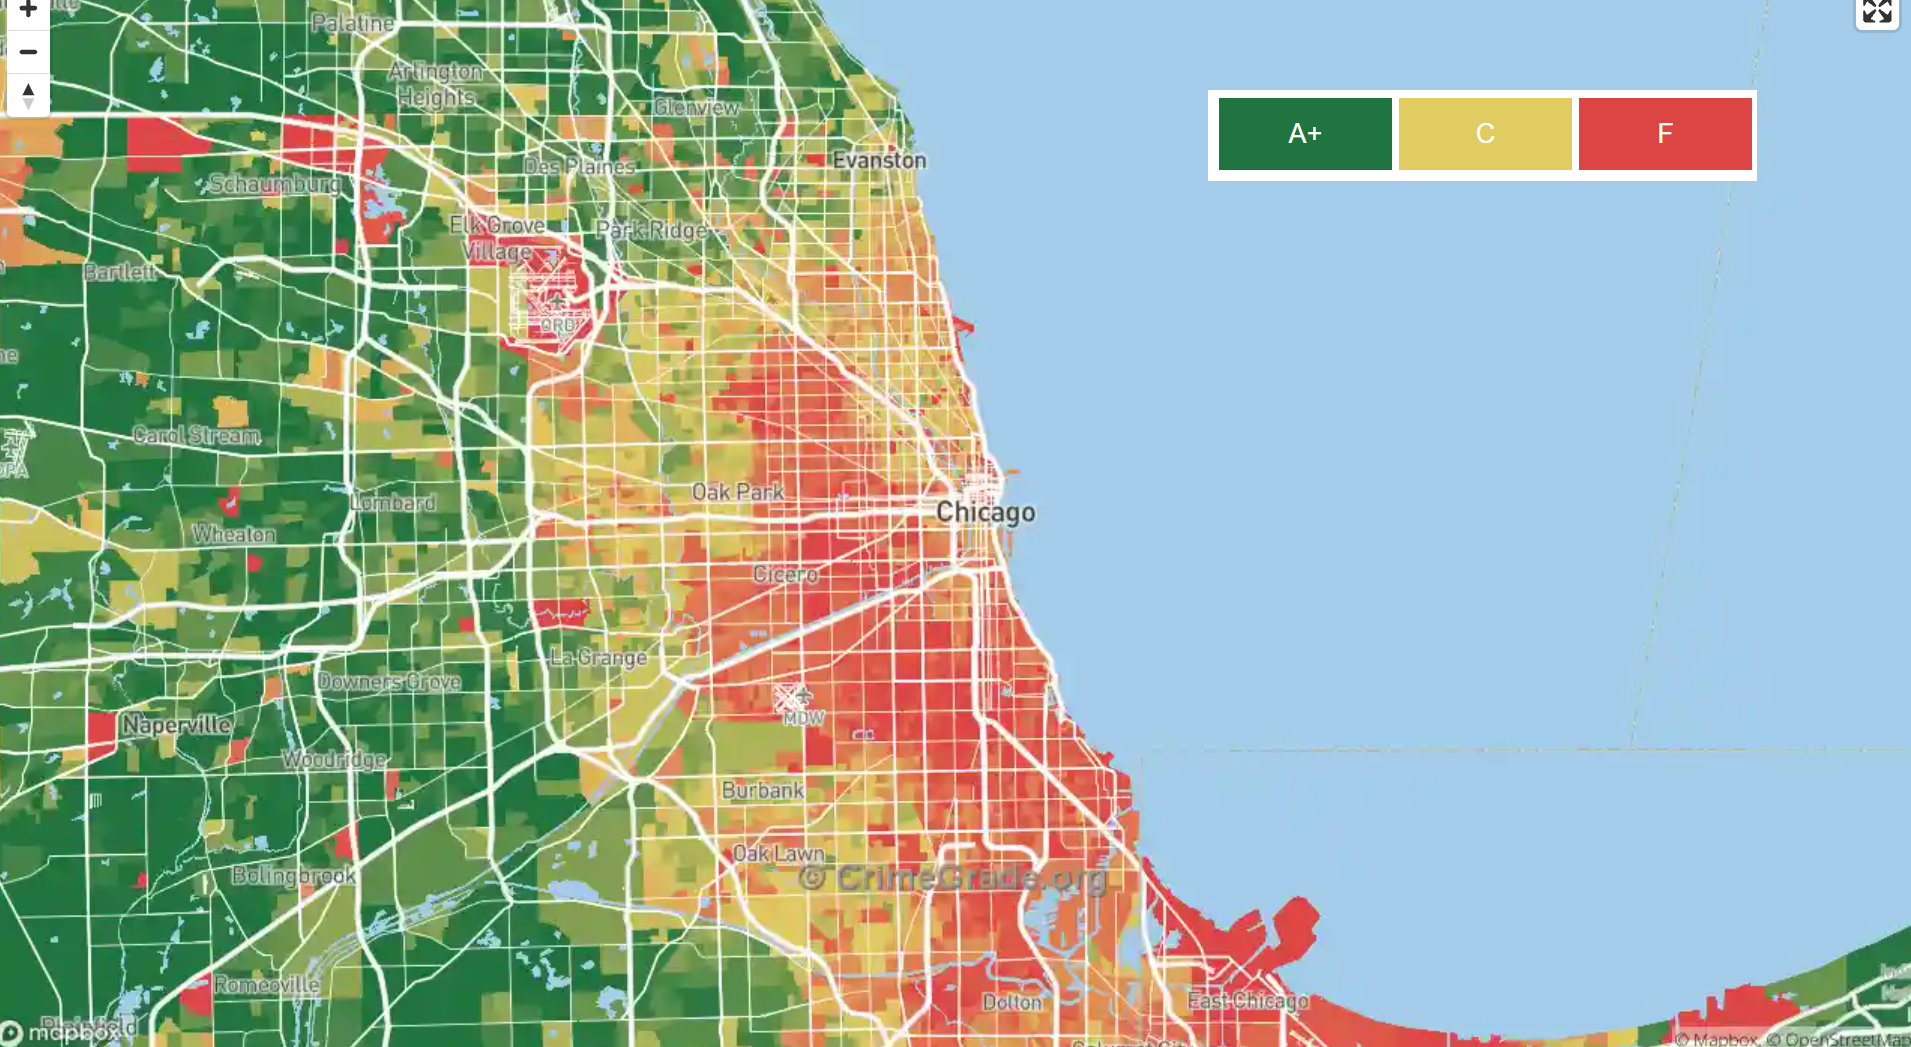
\includegraphics[scale=0.2]{figures/Crime_rate.png}
    \caption{Crime Distribution in Chicago Metro Area}
    \label{fig:Crime_rate.png}
\end{figure}
\end{itemize}
\end{frame}


%---------------------------------------------------------

\begin{frame}{Literature Review}
\begin{itemize}
 \item Public concern over safety $\longrightarrow$ one of the most important reasons why many choose not to use transit. 
\item Ecological approaches of analysing cause of crime: micro-environment of crime 
\item The relationship between transit system and crime is still in debate
\end{itemize}

\begin{figure}%
\hfill
\subfigure[Underpass platform at Lakewood station]{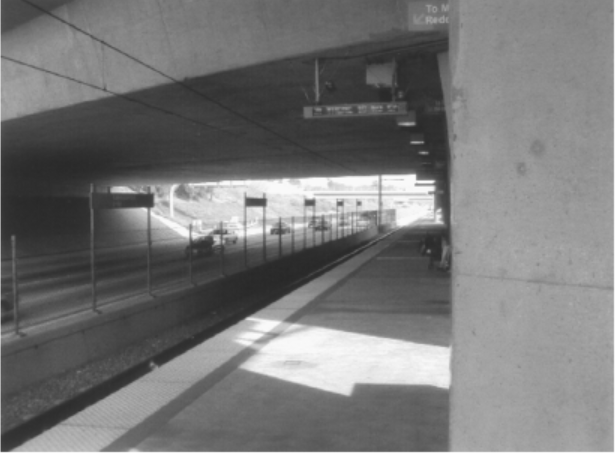
\includegraphics[scale=0.4]{figures/platform.png}}
\hfill
\subfigure[Overpass platform at Central Street in Chicago]{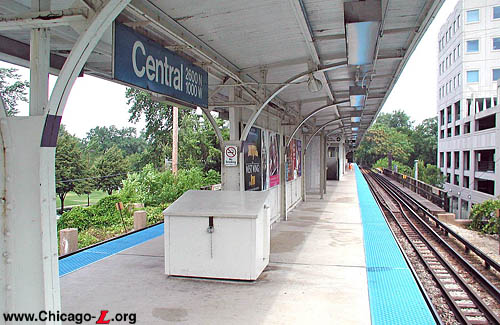
\includegraphics[scale=0.3]{figures/overpass.jpg}}
\hfill\hfill
\label{fig:station_samples}
\end{figure}

\end{frame}

%---------------------------------------------------------

\begin{comment}
\begin{frame}{Methodology}
\framesubtitle{Dataset}

\begin{itemize}
    \item \textbf{Crime records}\\ 
    \hspace{1cm} - Reported crime to CPD \\
    \hspace{1cm} - When, what, and where \\
    \hspace{1cm} - Data from 2010 to 2019 
    \item \textbf{Public transit information} \\
    \hspace{1cm} - \textbf{Chicago 'L'} and CTA bus \\
    \hspace{1cm} - Route/line, \textbf{station}/stop, average ridership
    \item \textbf{Chicago community area} \\
    \hspace{1cm} - Defined in 1920s \\
    \hspace{1cm} - Better than census tracts and wards \\
    \hspace{1cm} - Relatively homogeneous in one community
\end{itemize}

    
\end{frame}
\end{comment}

%---------------------------------------------------------

\begin{frame}{Methodology}
\framesubtitle{Data Source}

\begin{columns}
\begin{column}{0.5\textwidth}
\begin{itemize}
    \item \textbf{Crime records}
    \begin{itemize}
        \item Reported crime to CPD
        \item When, what, and where
        \item Data from 2010 to 2019
    \end{itemize}
    \item \textbf{Public transit information}
    \begin{itemize}
        \item \textbf{Chicago 'L'} and CTA bus
        \item Route/line, \textbf{station}/stop, average ridership
    \end{itemize}
    \item \textbf{Chicago community area}
    \begin{itemize}
        \item Defined in 1920s
        \item Better than census tracts and wards
        \item Relatively homogeneous in one community
    \end{itemize}
\end{itemize}
\end{column}
\begin{column}{0.5\textwidth}  
    \begin{center}
     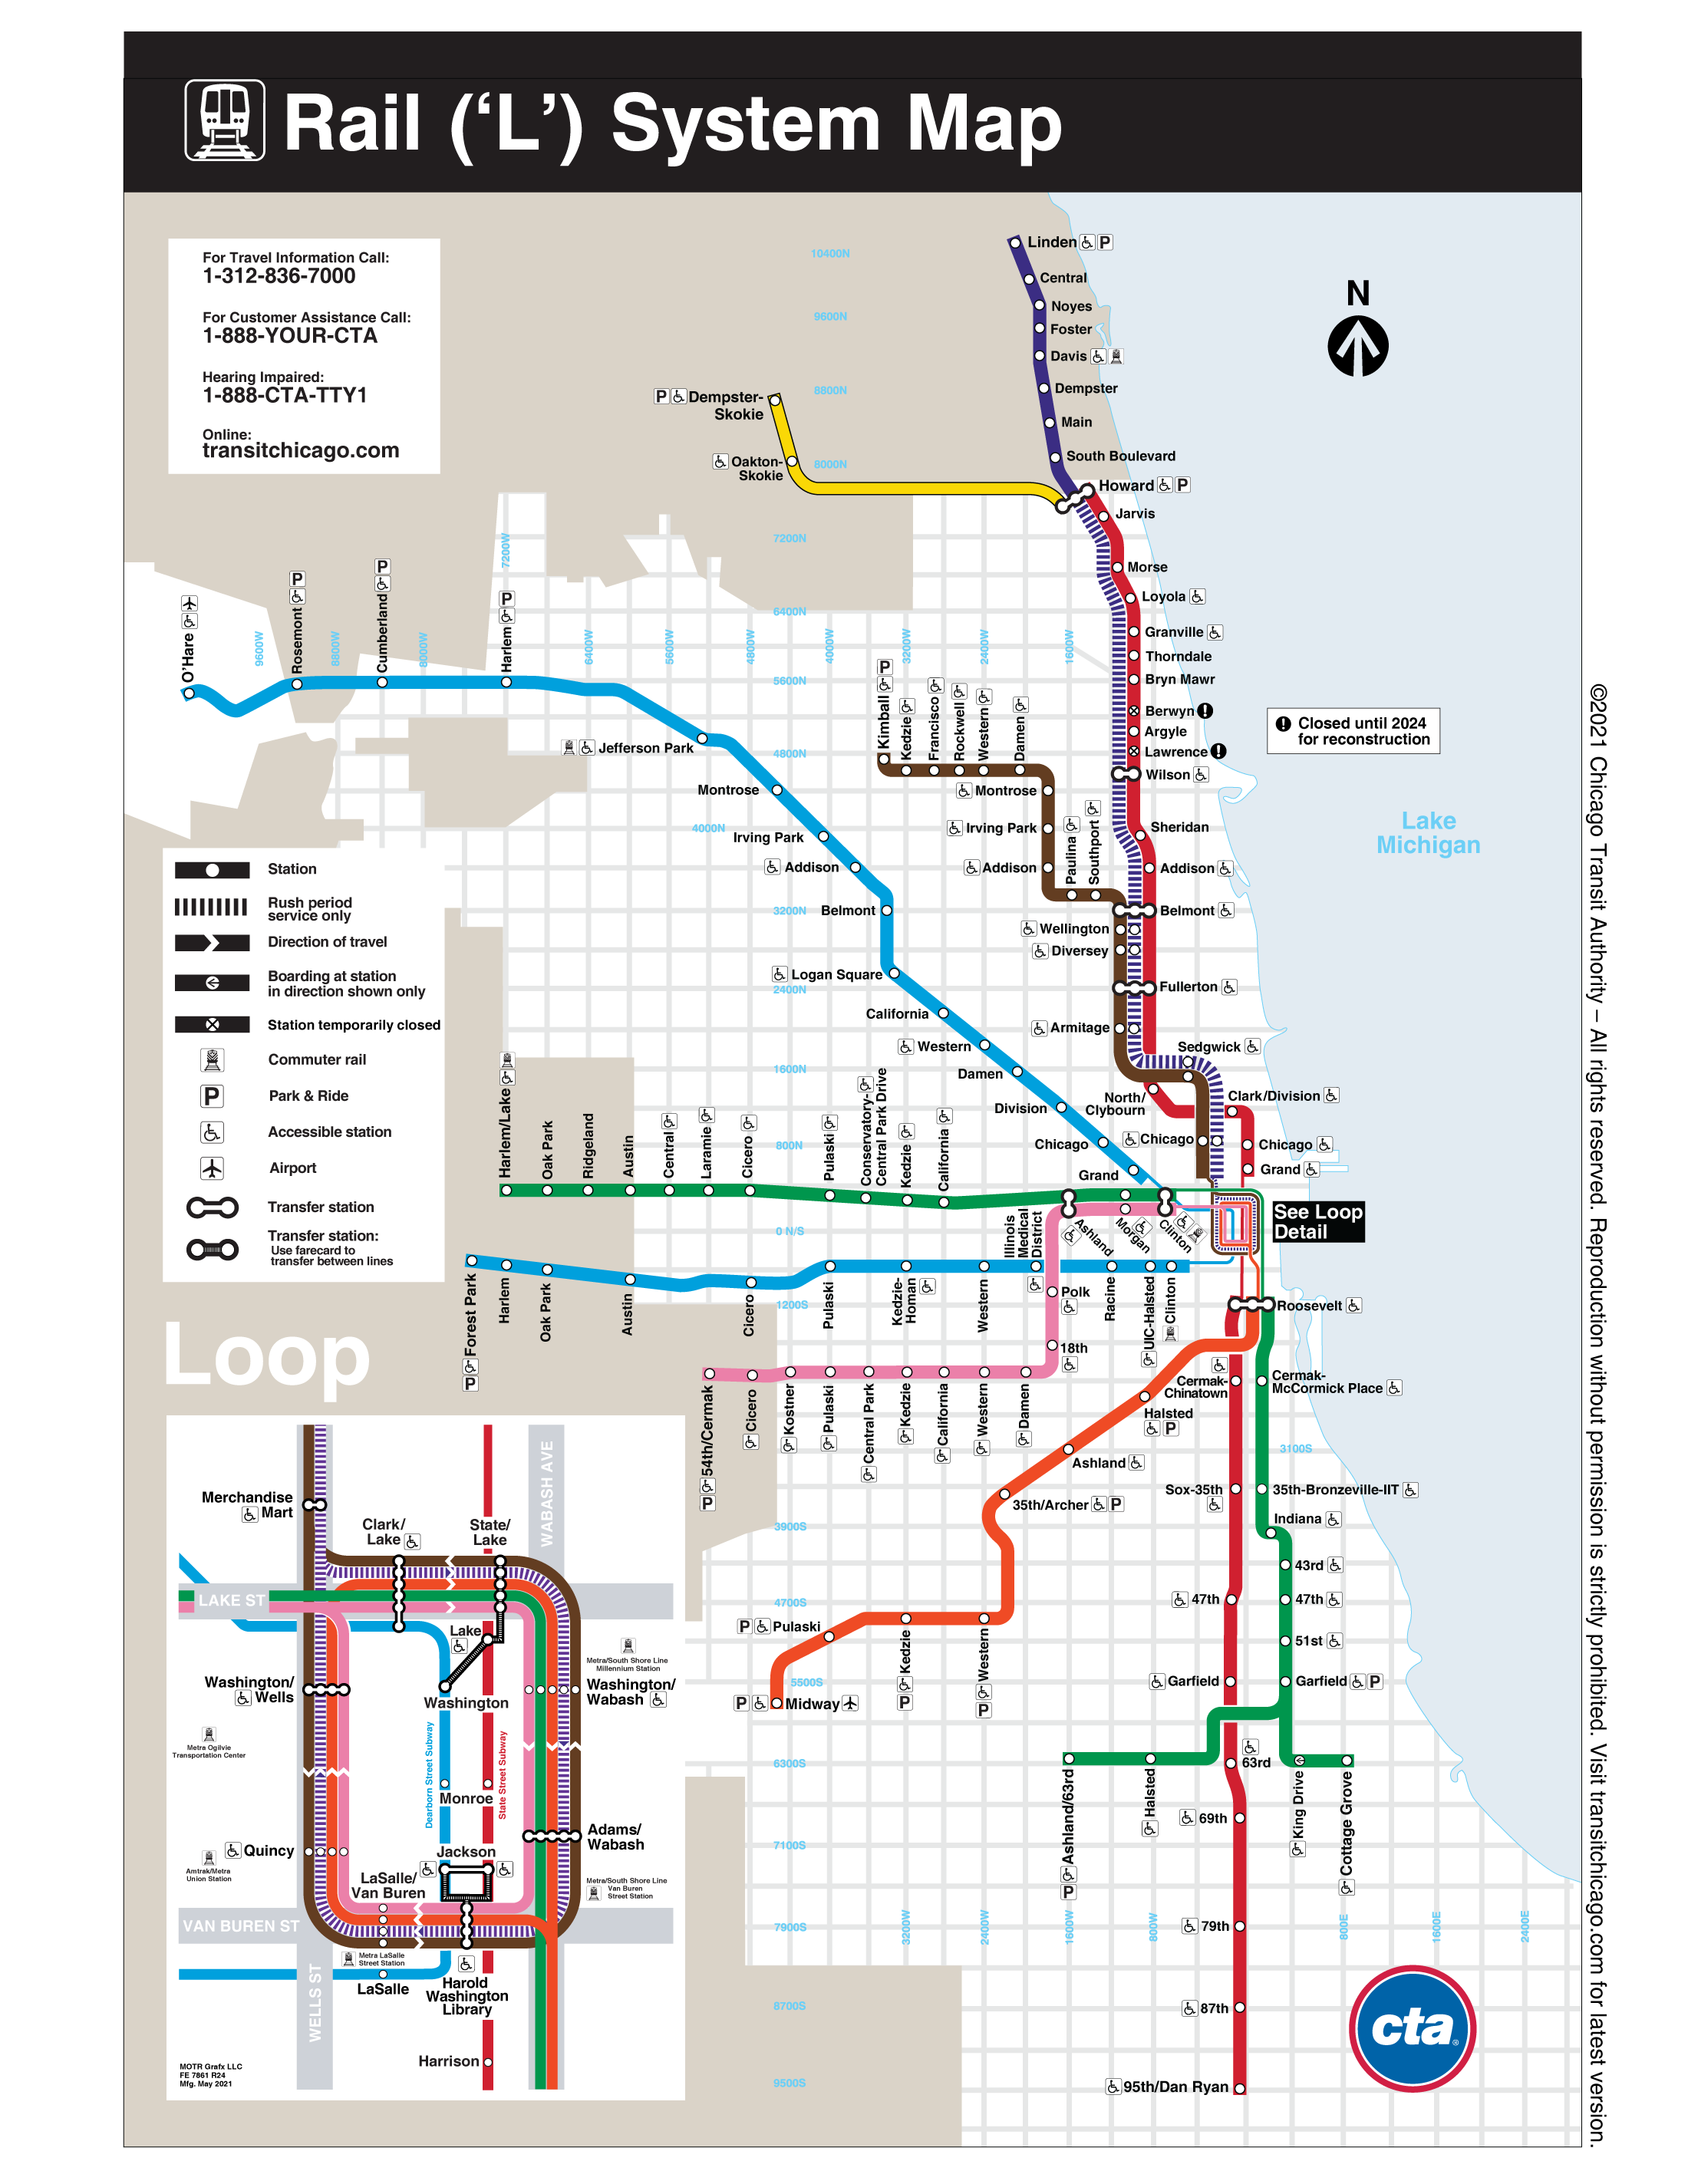
\includegraphics[width=0.9\textwidth]{figures/subway_map.png}
     \end{center}
\end{column}
\end{columns}


    
\end{frame}

%-----------------------------------------------

\begin{frame}{Methodology}
\framesubtitle{Spatial Data Processing}

\begin{figure}%
\hfill
\subfigure[Study Area]{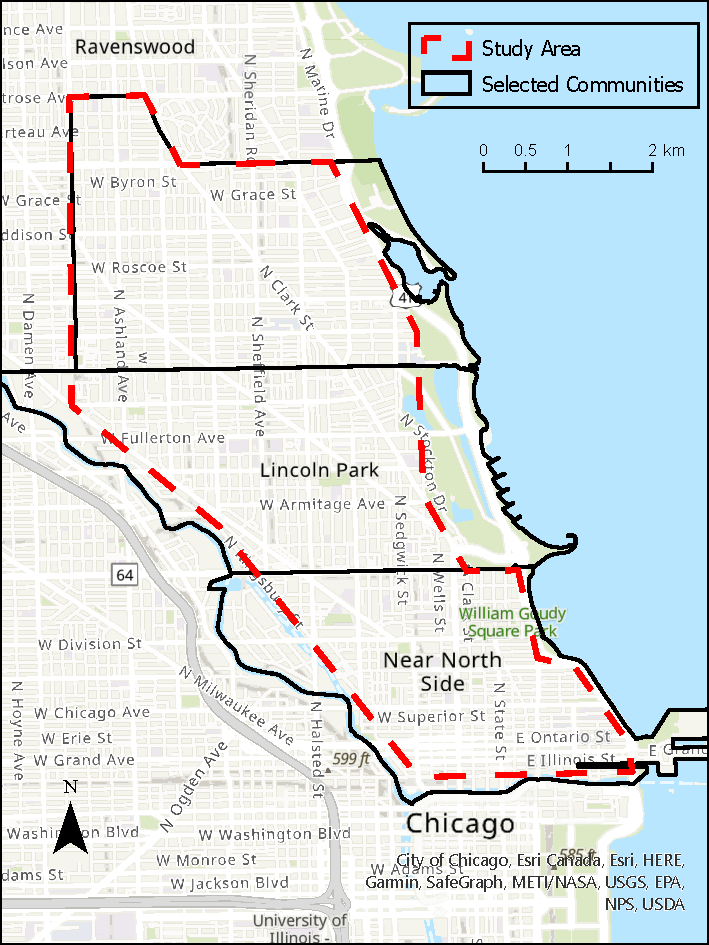
\includegraphics[scale=0.3]{figures/study_area.pdf}}
\hfill
\subfigure[Stations and Samples]{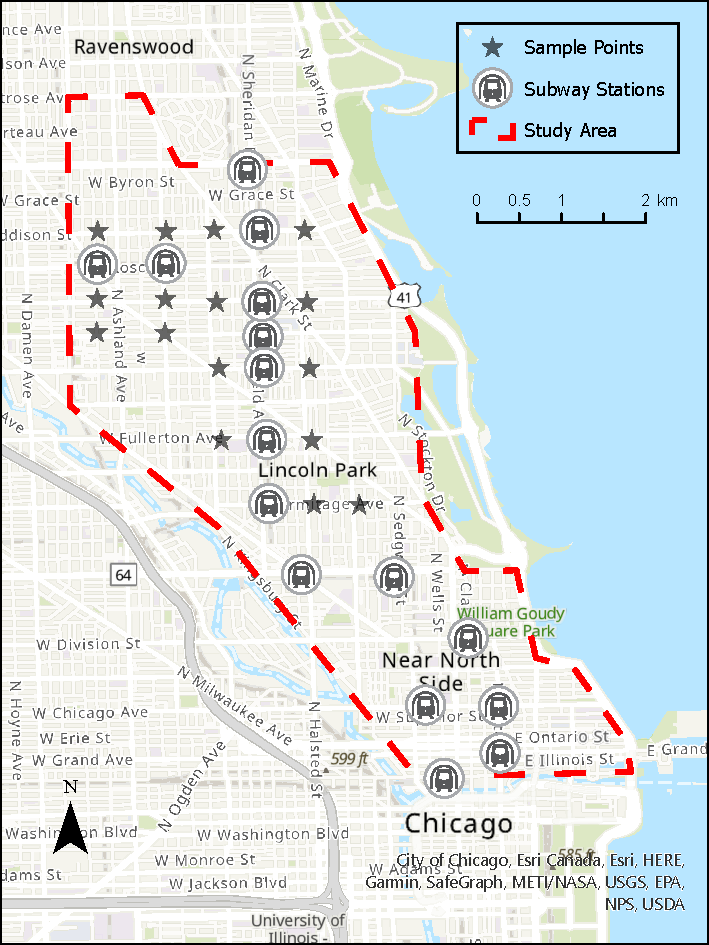
\includegraphics[scale=0.3]{figures/stations_and_samples.pdf}}
\hfill\hfill
\label{fig:station_samples}
\end{figure}

\centering{\footnotesize Socioeconomic scores for the selected communities}
\vspace{-0.2cm}
\begin{table} 
\centering
%\caption{Rankings of the selected communities in different socioeconomic characteristics.}
\label{tab:community_index}
\scalebox{0.6}{
\begin{tabular}{ l c c c c}
 \hline\hline
 Name & Density & Income Per Capita & Education Level & Overall Score \\ 
 \hline
 Lake View & 8 & 4 & 4 & 5\\  
 Lincoln Park & 2 & 2 & 2 & 2\\
 Near North Side & 1 & 1 & 1 & 1 \\
 \hline\hline
\end{tabular}
}
\end{table}

\end{frame}


%------------------------------------------------

\begin{frame}{Methodology}
\framesubtitle{Spatial Data Processing}

\begin{figure}
    \centering
    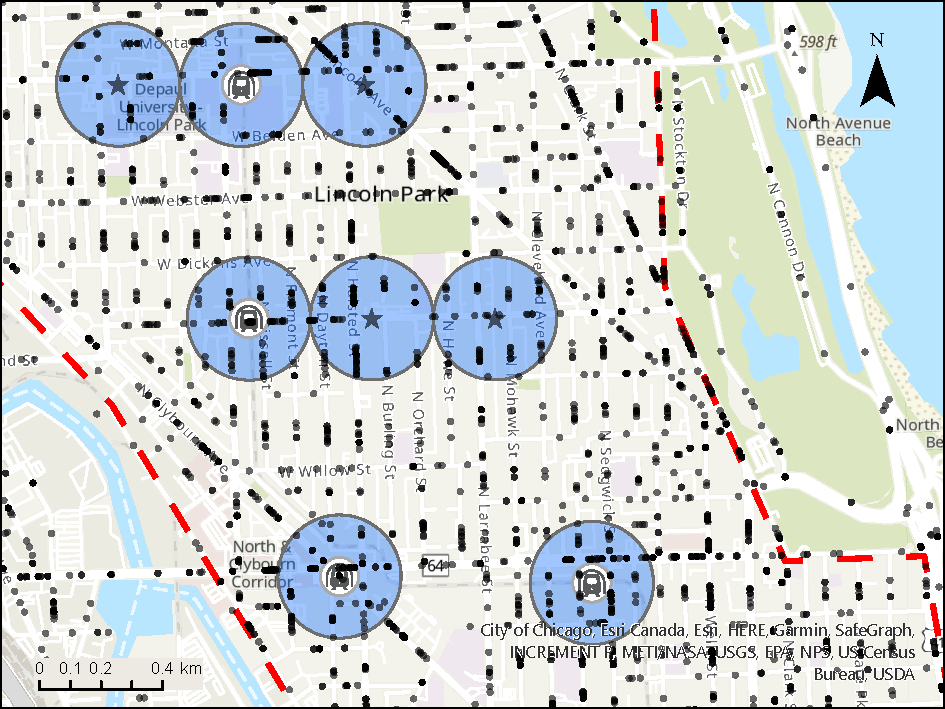
\includegraphics[width=8cm]{figures/circular_zone.pdf}
    \caption{200-Meter Buffers}
    \label{fig:circular_zone}
\end{figure}

\end{frame}

%------------------------------------------------

\begin{frame}{Methodology}
\framesubtitle{Spatial Data Processing}

\begin{table}[ht]
\centering
  \caption{An Overview of the Treatment Units} 
\scalebox{0.5}{
\begin{tabular}{rlllrrrrrrrrrrr}
  \hline\hline
 & station\_id & station\_name & community & 2010 & 2011 & 2012 & 2013 & 2014 & 2015 & 2016 & 2017 & 2018 & 2019 \\ 
  \hline
1 & 1210 & Wellington & LAKE VIEW & 108 & 128 & 120 & 111 &  95 &  90 &  85 &  93 &  97 &  72 \\ 
  2 & 1450 & Chicago & NEAR NORTH SIDE & 608 & 887 & 833 & 625 & 450 & 364 & 439 & 517 & 594 & 597 \\ 
  3 & 800 & Sedgwick & NEAR NORTH SIDE & 168 & 188 & 130 & 131 & 162 & 139 & 131 & 127 & 226 & 157 \\ 
  4 & 660 & Armitage & LINCOLN PARK & 126 & 134 & 102 & 121 &  80 &  78 &  81 & 102 & 121 &  94 \\ 
  5 & 1420 & Addison & LAKE VIEW & 263 & 229 & 313 & 236 & 194 & 213 & 255 & 191 & 241 & 179 \\ 
  $\vdots$ & $\vdots$ & $\vdots$ & $\vdots$ & $\vdots$ & $\vdots$ & $\vdots$ & $\vdots$ & $\vdots$ & $\vdots$ & $\vdots$ & $\vdots$ & $\vdots$ & $\vdots$ \\ 
   \hline\hline
\end{tabular}
}
\end{table}

\begin{table}[ht]
\centering
  \caption{An Overview of the Control Units} 
\scalebox{0.5}{
\begin{tabular}{rlllrrrrrrrrrr}
  \hline\hline
 & sampling\_id & coordinate\_x & coordinate\_y & 2010 & 2011 & 2012 & 2013 & 2014 & 2015 & 2016 & 2017 & 2018 & 2019 \\ 
  \hline
1 &   1 & 1164471.23 & 1924086.20 &  75 &  64 &  41 &  50 &  46 &  43 &  43 &  43 &  40 &  41 \\ 
  2 &   2 & 1164471.23 & 1921461.53 &  88 &  96 &  87 &  72 &  51 &  39 &  63 & 102 & 100 &  93 \\ 
  3 &   3 & 1164471.23 & 1920149.20 &  59 &  47 &  45 &  33 &  32 &  34 &  30 &  25 &  35 &  19 \\ 
  4 &   4 & 1166449.96 & 1924086.20 &  98 &  83 &  79 &  76 &  80 &  75 &  87 &  94 &  64 &  78 \\ 
  5 &   5 & 1166449.96 & 1921461.53 & 106 & 103 &  86 &  87 &  80 &  57 &  72 &  70 &  65 &  50 \\ 
  $\vdots$ & $\vdots$ & $\vdots$ & $\vdots$ & $\vdots$ & $\vdots$ & $\vdots$ & $\vdots$ & $\vdots$ & $\vdots$ & $\vdots$ & $\vdots$ & $\vdots$ \\
   \hline\hline
\end{tabular}
}
\end{table}

\end{frame}
%------------------------------------------------

\begin{frame}{Methodology}
\framesubtitle{Theoretical Framework}

\[\log Y_{it}=\beta + \delta D_{it} + \epsilon_{it} \]

\begin{itemize}
    \item $Y_{it}$: the number of crime cases at area $i$ during year $t$.
    \item $D_{it}$: treatment indicator, which is equal to 1 if there is a transit within area $i$ in year $t$, and 0 otherwise.
    \item $\delta$: the average treatment effect averaged over all years.
    \item $\epsilon_{it}$: the error term.
\end{itemize}


\end{frame}

%------------------------------------------------

\begin{frame}{Methodology}
\framesubtitle{Assumption Check}


\begin{figure}
    \centering
    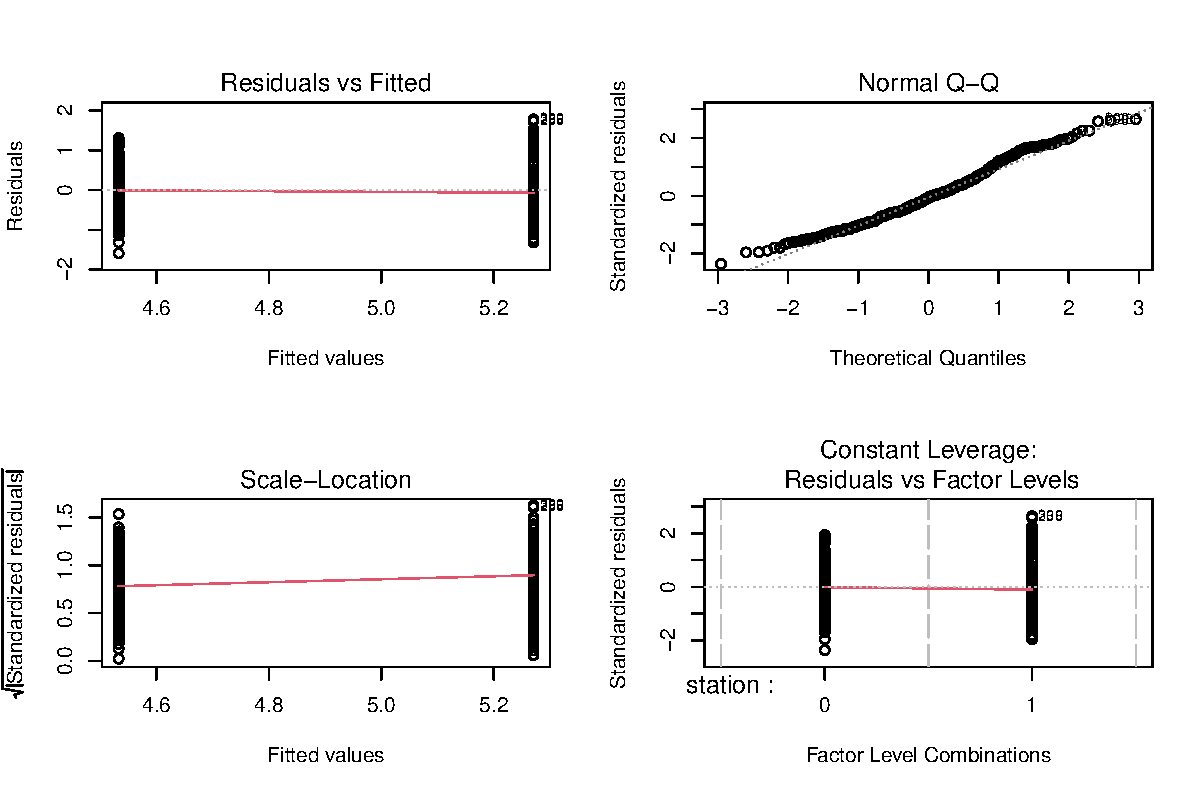
\includegraphics[scale=0.5]{figures/logplot.pdf}
    \caption{Diagnostic Plots}
    \label{fig:diagnostic}
\end{figure}


\end{frame}




%------------------------------------------------

\begin{frame}{Results}



\begin{figure}
    \centering
    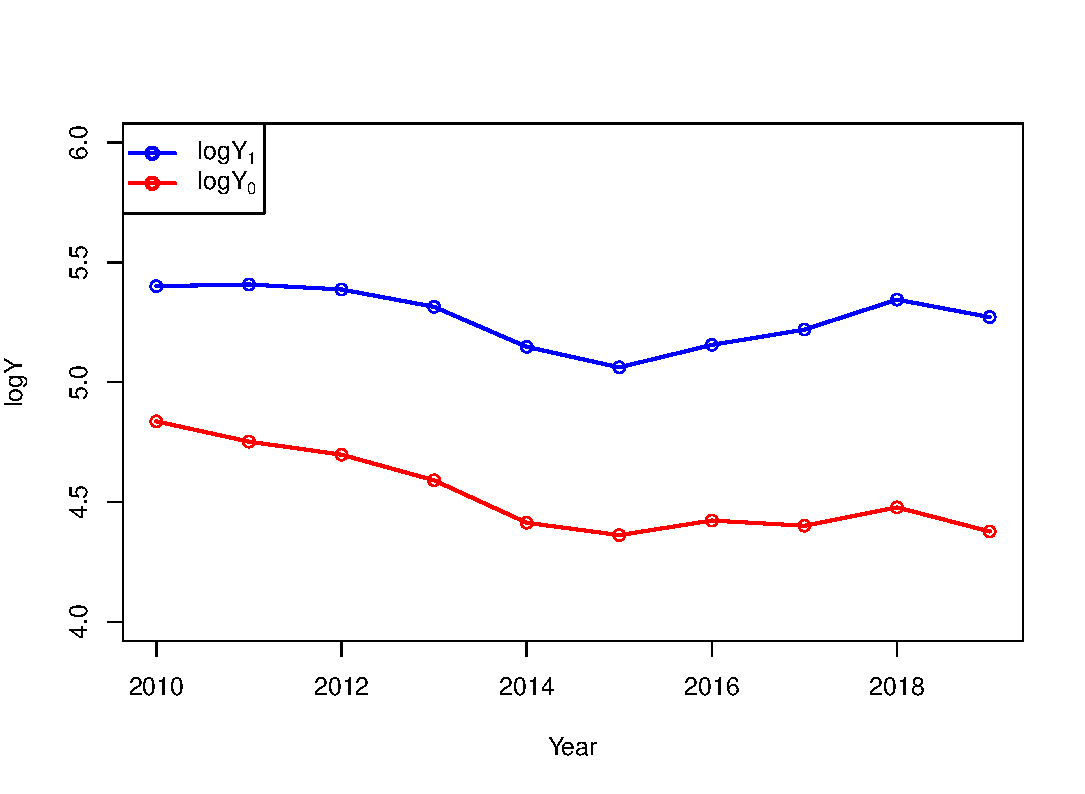
\includegraphics[scale=0.4]{figures/lncrime-year1.pdf}
    \caption{log(Crime) vs. Year}
    \label{fig:lncrime-year}
\end{figure}



\end{frame}

%------------------------------------------------


\begin{frame}{Results}

\begin{figure}
    \centering
    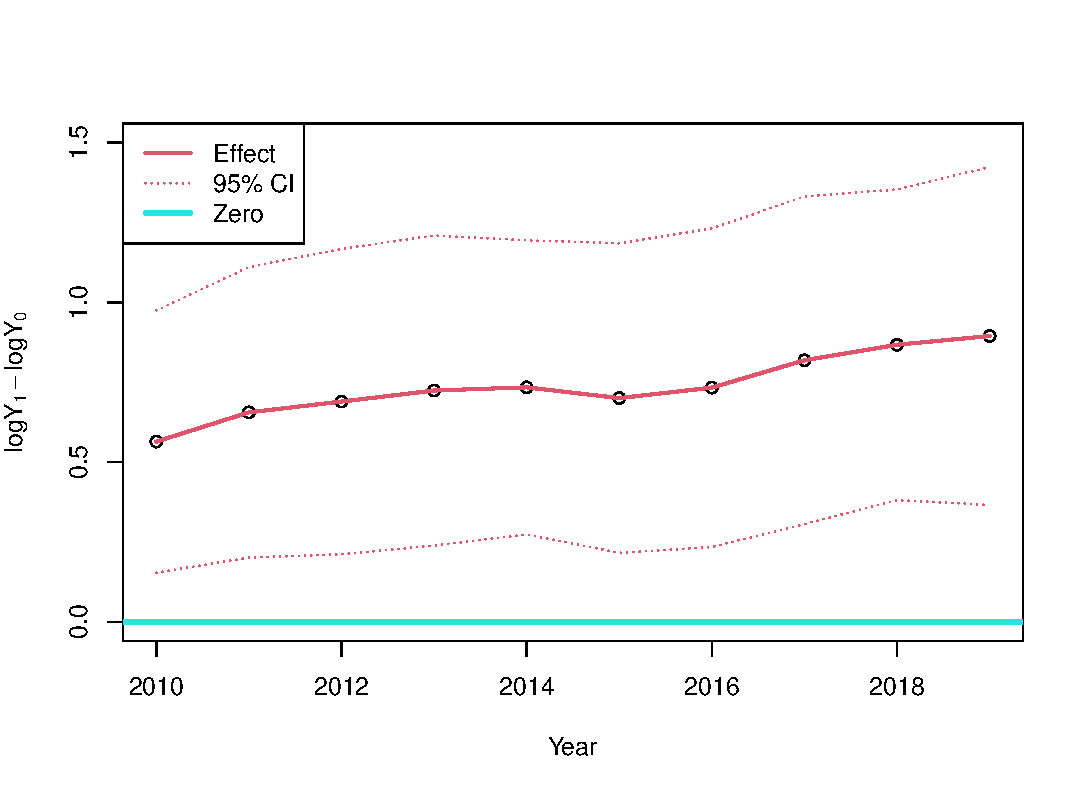
\includegraphics[scale=0.4]{figures/ate-year1.pdf}
    \caption{Effect vs. Year}
    \label{fig:ate-year}
\end{figure}


\end{frame}

%------------------------------------------------

\begin{frame}{Results}
\begin{table}[!htbp] \centering 
  \caption{Average Treatment Effect Averaged over 10 Years} 
  \label{} 
  \footnotesize
\begin{tabular}{@{\extracolsep{5pt}}lc} 
\\[-1.8ex]\hline 
\hline \\[-1.8ex] 
 & \multicolumn{1}{c}{\textit{Dependent variable:}} \\ 
\cline{2-2} 
\\[-1.8ex] & lncrime \\ 
\hline \\[-1.8ex] 
 station1 & 0.738$^{***}$ \\ 
  & (0.076) \\ 
  & \\ 
 Constant & 4.533$^{***}$ \\ 
  & (0.053) \\ 
  & \\ 
\hline \\[-1.8ex] 
Observations & 320 \\ 
R$^{2}$ & 0.231 \\ 
\hline 
\hline \\[-1.8ex] 
\textit{Note:}  & \multicolumn{1}{r}{$^{*}$p$<$0.1; $^{**}$p$<$0.05; $^{***}$p$<$0.01} \\ 
\end{tabular} 
\end{table} 

\begin{itemize}
    \item Positive effect of station on local crime
    % \item Effect size is 0.738 in log terms
    \item Effect on $Y$ is 109.2\% ($e^{0.738}-1$)
\end{itemize}

\end{frame}

%------------------------------------------------



\begin{frame}{Conclusion}

\textbf{Causal channel}: 
\begin{itemize}
    \item Station $\to$ Larger commuter flow $\to$ More crime opportunities
\end{itemize}

\vspace{1em}

Three perspectives:

\begin{itemize}
    \item Policy-makers: hard to monitor criminal behaviors at stations
    \item Criminals: easy to escape at stations
    \item Overall: more potential victims and offenders at stations
\end{itemize}




\end{frame}

%----------------------------------------
\begin{frame}

\begin{center}
\begin{huge}
Thank you for your attention!

\vspace{4mm}
Any questions?
\end{huge}

\end{center}


\end{frame}


\end{document}